\subsection{Resource-Constrained Project Scheduling Problem} \label{subsec:MRCPSP_RCPSP}

% Einfach

Eines der am meisten behandelten Optimierungsprobleme stellt das \ac{rcpsp} dar. Das grundlegende \ac{rcpsp} behandelt das Finden von Schedules (dt. Zeitplänen) bei einem gegebenen Projektplan. Ein Projekt besteht aus einer Menge von Aktivitäten $J = \{ 0, ..., j, j + 1 \}$, wobei es sich $J_0$ und $J_{j+1}$ um Dummy-Aktivitäten handeln, welche den Projektstart bzw. das Projektende repräsentieren. Aktivitäten können untereinander in Beziehung stehen, sodass eine Aktivität $j \in J$ erst gestartet werden kann, wenn alle seine Vorgänger $P(j) \in 2^J$ fertiggestellt wurden. Diese besitzen im Grundproblem zudem eine feste Dauer $d_j \in \mathbb{N}_0$ und Ressourcenanforderungen $r_{j,k} \in \mathbb{N}_0$. Bei den Ressourcen wird zwischen erneuerbaren Ressourcenarten $K = \{1, ..., R\}$ unterschieden. Alle Ressourcenarten stehen innerhalb eines Projektes nur in limitierter Anzahl $R_{k} \in \mathbb{N}$ zur Verfügung, welche während der Projektausführung über die Aktivitäten aufgeteilt werden müssen. Für die Projektstart- und Ende-Aktivitäten gelten zudem $\forall \, k \in K: r_{j,k} = 0$ und $d_j = 0$. Diese Restriktion zeigt auf, dass keine Ressourcen- und Zeitanforderungen für die Aktivitäten gegeben sind. Zudem dürfen Aktivitäten nicht bei der Ausführung unterbrochen werden. \cite[vgl.][S. 1 ff.]{kolisch_heuristic_1998}. \\

Das Ziel des \ac{rcpsp} liegt darin, den Zeitplan mit der minimalsten Makespan (zu dt. Projektausführungsdauer) zu bestimmen. Formal wird die Zielfunktion des \ac{rcpsp} von \cite[S. 1]{kolisch_heuristic_1998} vergleichsweise wie folgt beschrieben:
\begin{align}
    \min \, F_{n+1} = \min \, C_{max} & \qquad \textit{es muss gelten:} \label{align:rcpsp_goal} \\
    \forall j \in J, h \in P_j:\, & F_h \leq F_j - d_j \label{align:rcpsp_constraint1} \\
    \forall k \in K, t \geq 0:\, & \sum_{j \in A(t)} r_{j,k} \leq R_k  \label{align:rcpsp_constraint2}
\end{align}
Die Menge der zum Zeitpunkt $t$ ausgeführten Aktivitäten wird über $A(t)$ angegeben. $F_j$ entspricht der Endzeit einer Aktivität $j \in J$. Eine Aktivität kann erst gestartet werden, wenn alle unmittelbaren Vorgänger abgeschlossen wurden (vgl. Formel \ref{align:rcpsp_constraint1}). Formel \ref{align:rcpsp_constraint2} gewährleistet, dass die Kapazitäten von den erneuerbaren Ressourcen zu jedem Zeitpunkt nicht überschritten werden dürfen. 

\begin{figure}[H]
    \centering
    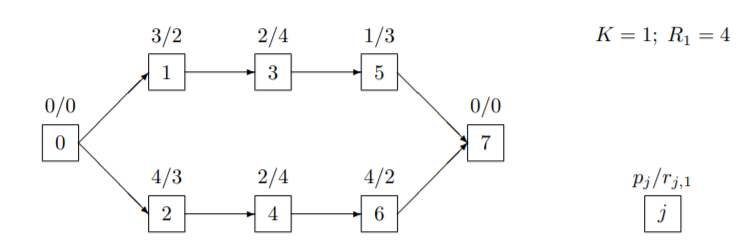
\includegraphics[width=1\textwidth]{assets/img/02_Grundlagen/ExampleProjectRCPSP_Plan.png}
    \caption{Graphen-Darstellung eines \ac{rcpsp} Beispiel-Projektplans mit $|J| = 8$ Aktivitäten} 
    \label{img:example_rcpsp}
    \source{\cite[][S. 2]{kolisch_heuristic_1998}}
\end{figure}

Abbildung \ref{img:example_rcpsp} stellt einen beispielhaften Projektplan mit $|J| = 8$ Aktivitäten als Knoten samt deren Ressourcen- und Zeitanforderungen dar. Diese stehen oberhalb der Knoten in der Schreibweise $d_j / r_{r,i}$. $J_0$ und $J_7$ entsprechen den Dummyknoten, welche keine Ressourcen- und Zeitanforderungen aufweisen. Die Kanten zeigen Beziehungen zu den Nachfolgeaktivitäten auf. Zudem steht eine erneuerbare Ressourcenart mit einer Kapazität von 4 Mengeneinheiten ($R_1 = 4$) zur Verfügung. 

\begin{figure}[H]
    \centering
    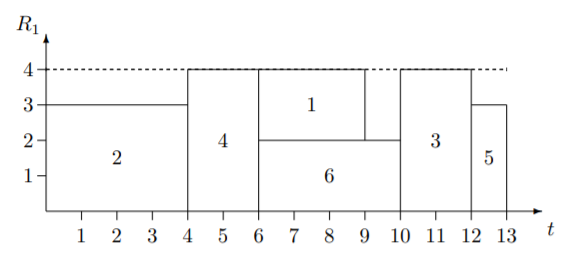
\includegraphics[width=0.8\textwidth]{assets/img/02_Grundlagen/ExampleProjectRCPSP_Schedule.png}
    \caption{Möglicher Zeitplan zum \ac{rcpsp} Beispiel-Projektplan} 
    \label{img:example_rcpsp_schedule}
    \source{\cite[][S. 2]{kolisch_heuristic_1998}}
\end{figure}
Ein möglicher Zeitplan zu dem Beispiel-Projektplan lässt sich in der Abbildung \ref{img:example_rcpsp_schedule} darstellen. Hierbei werden die Ressourcenanforderungen der Aktivitäten mit Berücksichtigung der Abhängigkeiten auf der Zeitachse gemäß deren Dauer zugeordnet. Die gestrichelte, horizontale Linie entspricht der maximalen Kapazität für die Ressource $K_1$, welche $R_1 = 4$ gleichkommt. Diese darf bei der Zeitplanung nicht überschritten werden. Der Makespan (dt. Zykluszeit) $C_{max} = 13$ des Zeitplans lässt sich über der Belegung der erneuerbaren Ressourcenarten über den Endzeitpunkt der letzten Aktivität $J_{j+1}$ ablesen. \\

Das \ac{rcpsp} wird als eine generalisierte Form des \ac{jsp} angesehen, welches als $\mathcal{NP}$-hartes Problem  klassifiziert wurde \cite[vgl.][S. 2]{kolisch_heuristic_1998}. Konkret bedeutet dies, dass das Finden des besten Zeitplans nur bei einem kleinen Lösungs-raum deterministisch über Bruteforcing möglich ist. Bei komplexeren Lösungsräumen sind jedoch zu viele Möglichkeiten vorhanden, als dass in absehbarer Zeit alle Kombinationen betrachtet werden können. \\
% Nicht-erneuerbare Ressourcen stellen zudem ein weiteres Problem dar, denn ungültige Lösungen können auftreten wenn zu einem Zeitpunkt keine nicht-erneuerbaren Ressourcen mehr zur Verfügung stehen. \\
\\
Für das zugrunde liegende Problem wurden (Meta-)Heuristiken und weitere intelligente Verfahren eingeführt, welche zur Findung von adäquaten Zeitplänen beim \ac{rcpsp} eingesetzt werden können \cite[vgl.][S. 2]{kolisch_heuristic_1998}. Der Fokus dieser Masterarbeit liegt bei den Metaheuristiken, welche im Abschnitt \ref{sec:Metaheuristiken} eingeführt werden.
